\subsection{Gyroskop}\label{sec:gyroskop}
In der Teststation sollen Tests durchgeführt werden, bei denen sich der Satellit rotiert. Der Satellit sollte sich in alle Richtungen drehen können, denn nur so können die Gyro Sensoren komplett und genau getestet werden. Da sich der Satellit später im All willkürlich rotiert, bringt eine konstante Rotation um nur eine Achse nichts. Aus diesem Grund wird ein sogenanntes Gyroskop oder auch Kreiselinstrument verwendet. Ein Gyroskop kann ein Objekt gleichzeitig in alle Richtungen (x,y,z) drehen. Es besteht aus 3 Ringen, der äußerste Ring wird mit einem Stepper Motor um die X-Achse in Bewegung gesetzt, der Mittlere Ring dreht sich dann mit dem Eigengewicht um die Y-Achse und der innerste Ring ist in unserer Anwendung der Satellit. \\ 
\vspace{3mm}
Um die Ringe in einer Höhe von 30cm zu halten, braucht es 2 Halterungen. Diese Halterungen werden aus Flachstangen, die eine Stärke von 8mm und einer Breite von 20mm haben, geschweißt. Dazu sind folgende Flachstange notwendig. \\
\vspace{3mm}
\begin{table}[H]
    \centering
    \begin{tabular}{ | c | c | } 
  \hline
   \textbf{Bezeichnung} & \textbf{Stückzahl}\\ 
  \hline
   Flachstange 5cm & 4\\ 
  \hline
   Flachstange 20cm & 2 \\ 
  \hline
  Flachstange 25cm & 4 \\ 
  \hline
  Flachstange 10cm & 2 \\ 
  \hline
  Flachstange 30cm & 2 \\ 
  \hline
\end{tabular}
    \caption{Stückliste Halterung Gyroskop}
\end{table}
\vspace{3mm}
\begin{figure}[H]
    \centering
    \begin{subfigure}[b]{0.4\textwidth}
        \centering
        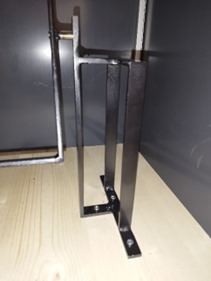
\includegraphics[width=\textwidth]{image/gyroskop1.jpeg}
        
        \label{fig:bild1}
    \end{subfigure}
    \hfill
    \begin{subfigure}[b]{0.4\textwidth}
        \centering
        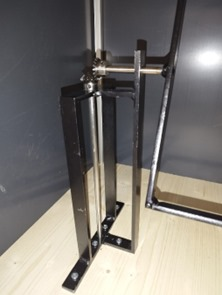
\includegraphics[width=\textwidth]{image/gyroskop2.jpeg}
        
        \label{fig:bild2}
    \end{subfigure}
    \caption{Halterung Gyroskop}
    \label{fig:zwei_bilder}
\end{figure}
\vspace{3mm}

\textbf{Komplette Zusammenschaltung Gyroskop}\\
\vspace{3mm}
Das Relais steuert das Netzteil, welches die Spannung für den Treiber liefert. Der Treiber bekommt Signale vom Raspberry Pi und steuert mit denen die Wicklungen vom Motor. \\
\vspace{3mm}
\begin{figure}[H]
    \centering
    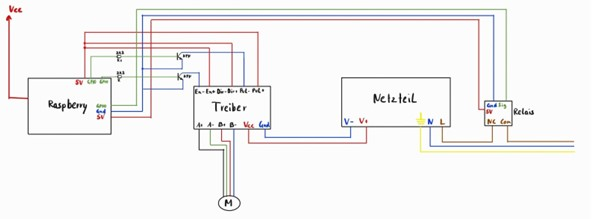
\includegraphics{image/zusammengyros.jpg}
    \caption{Zusammenschaltung Gyroskop}
    \label{fig:enter-label}
\end{figure}


\subsubsection{Motor}
Als Motor wurde der STEPPERONLINE Nema 17 Schrittmotor\autocite{Schrittmotor} gewählt, der speziell für 3D-Drucker und CNC-Reprap-Maschinen konzipiert ist. Mit einem Drehmoment von 59 Ncm, einer Betriebsspannung von 24V, einem Strom von 2A und einem Schrittwinkel von 1.8 Grad pro Schritt gewährleistet er präzise Bewegungssteuerung. Das 4-Draht-Design und das beiliegende 1 Meter lange Kabel mit Verbinder ermöglichen eine einfache Integration in unsere Teststation. Dieser Schrittmotor ist optimal für DIY-Projekte und Anwendungen mit hohen Anforderungen an Präzision und Steuerung von Bewegungen.
\begin{figure}[H]
    \centering
    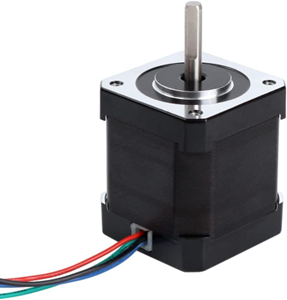
\includegraphics{image/schrittmotor.png}
    \caption{Schrittmotor}
    \label{fig:enter-label}
\end{figure}
Befestigung am Gyroskop und 5V Steuerung FETT:\\
\vspace{3mm}
Zuerst war geplant, den Ring im Gyroskop über eine Antriebsstange zu betreiben, dazu wäre ein 90° Umlenkung mit Zahnrädern notwendig gewesen. Da die Getriebe Stange über 30cm lang ist und nicht präzise zentriert ist, ist es schwierig, ein leicht gängiger Antrieb zu erhalten. Aus diesem Grund wird der Motor direkt an dem Linker Steher befestigt. \\
\vspace{3mm}
\begin{figure}[H]
    \centering
    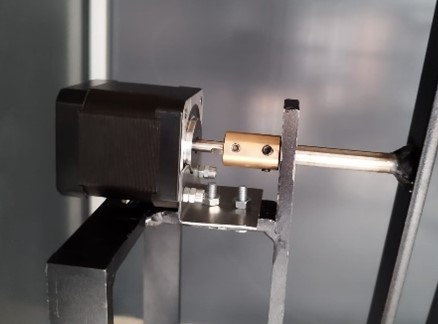
\includegraphics[scale=1.1]{image/motorgyros.jpg}
    \caption{Motor am Gyroskop}
    \label{fig:enter-label}
\end{figure}
\\
\vspace{2mm}
Die GPIO-Pins\label{sec: 5V} vom Raspberry Pi haben eine Ausgangsspannung von 3.3V. Für den Motor Treiber TB6600 wird aber eine Signalspannung von 5V benötigt. Mit einem NPN-Transistor und einem 2k2 Widerstand wird eine Ausgangsspannung von 5V erzeugt. Diese Zusammenschaltung wird auch Emitter Schaltung bezeichnet. Die Basis des bipolaren NPN-Transistors wird über einen Vorwiderstand mit dem Ausgangssignal eines GPIO-Pins vom Raspberry verbunden, während der Emitter mit dem 5V Ausgang vom Raspberry verbunden ist. Am Emitter ist zu gleich das Ausgangssignal mit nun 5V. Dieser wird mit dem Eingang vom Treiber verbunden. 
\subsubsection{Motor-Treiber}
Da man den Motor nicht direkt mit einem Raspberry steuern kann, braucht es einen Motortreiber. Der Twotrees DM542 5.6A Schrittmotortreiber\autocite{Treiber} ist ein leistungsstarker Treiber für 2-Phasen-Schrittmotoren, wie unser Motor, der verwendet wird. Hier ist eine kurze technische Produktbeschreibung:\\
\vspace{3mm}
Eigenschaften:
\begin{itemize}
    \item Leistung: Der Treiber unterstützt Motoren mit bis zu 5.6A Stromversorgung.
    \item Betriebsspannung: Geeignet für Gleichstromquellen im Bereich von 18-48V.
    \item Schrittauflösung: Präzise Mikroschrittsteuerung für genaue Positionierung.
    \item Phasen: Entwickelt für 2-Phasen-Schrittmotoren.
    \item Peak-Strom: Bietet einen Spitzenstrom von bis zu 4.2A für verbesserte Motorleistung.
\end{itemize}
\vspace{3mm}
Schutz und Zuverlässigkeit:
\begin{itemize}
    \item Überstromschutz: Der Treiber ist mit einem Überstromschutz ausgestattet, der den Motor vor Schäden durch zu hohe Ströme schützt.
    \item Wärmeschutz: Integrierter Schutzmechanismus gegen Überhitzung für eine zuverlässige Langzeitnutzung. So können wir die Tests lang genug durchführen.
\end{itemize}
Der Twotrees DM542 5.6A Schrittmotortreiber bietet eine leistungsstarke und zuverlässige Lösung für die Steuerung von 2-Phasen-Schrittmotoren in anspruchsvollen Anwendungen. Mit Funktionen wie Überstromschutz, Wärmeschutz und Mikroschrittsteuerung ist er eine geeignete Wahl für unsere Gyroskop Ansteuerung.
\begin{figure}[H]
    \centering
    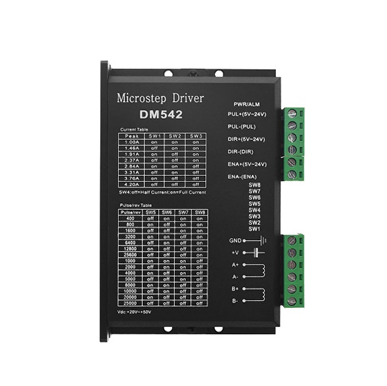
\includegraphics{image/treiber.png}
    \caption{Motor-Treiber}
    \label{fig:enter-label}
\end{figure}

\subsubsection{Netzteil}
Der Motortreiber muss man mit mindestens 9V DC versorgen. Diese Spannung wird mit einem Netzteil erzeugt. Das MeanWell\autocite{MeanWell} LRS-100-24 ist ein industrielles Netzteil mit 108W Leistung, einer Ausgangsspannung von 24V und 4,5A Ausgangsstrom. Es ist für den zuverlässigen Einsatz in industriellen Anwendungen wie Steuerungen und LED-Beleuchtungen konzipiert. Mit integriertem Überlast- und Kurzschlussschutz bietet es eine effiziente und sichere Stromversorgungslösung. Seine robuste Bauweise und Kompaktheit machen es ideal für anspruchsvolle Umgebungen mit begrenztem Platz.
\vspace{5mm}
\begin{figure}[H]
    \centering
    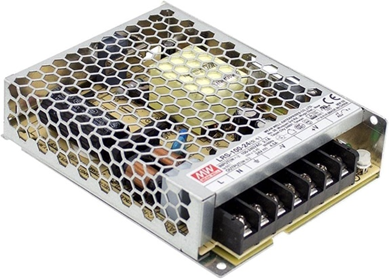
\includegraphics{image/Netzteil.png}
    \caption{Netzteil}
    \label{fig:enter-label}
\end{figure}

\newpage
\subsubsection{Relais}\label{sec:relai}
\begin{figwindow}[1,r,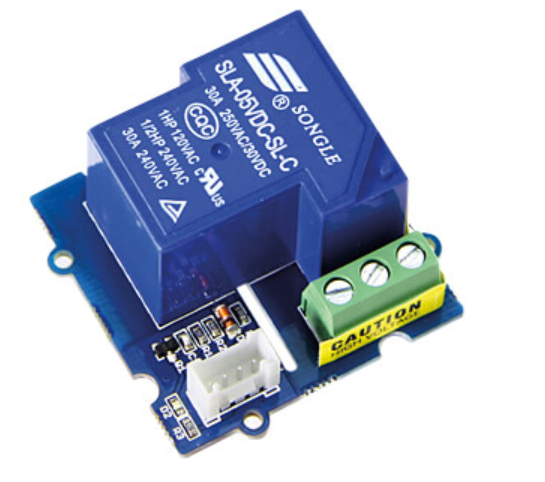
\includegraphics[scale=0.5]{image/relai.jpg.png},{Relais\autocite{Relais}}]
Mit einem Relais kann man mit kleinen Spannungen große Spannungen schalten. Ein Relais\autocite{Relais} besteht aus einer Spule und einem beweglichen Kontakt. Wenn Strom durch die Spule fließt, erzeugt sie ein Magnetfeld, das den Kontakt beeinflusst. Dadurch ändert sich der Zustand des Schaltkontakts, und ein elektrischer Pfad wird geöffnet oder geschlossen. Relais dienen dazu, mit einem schwachen Steuersignal einen starken elektrischen Stromkreis zu steuern oder zu schalten. Relais werden in unserer DA verwendet, um mit dem Raspberry Netzspannungen zu schalten. 
Für unsere Anwendung brauchen wir das GRV RELAY SPDT30, dieses ist ein hochwertiges einpoliges Zweiwege-Relais mit hoher\\ Schaltleistung. Es ist für Betriebsspannungen von 4,75 bis 5,25 V und Schaltströme von bis zu 30 A bei 250 V AC oder 30 V DC ausgelegt. Das Relais ist kompatibel mit den Schnittstellen vom Raspberry Pi, verfügt über eine schnelle Einschaltzeit von maximal 15ms und eine Betriebstemperatur von -25 bis +75°C.  Eingesetzt wird es in der Teststation für die Steuerung des Netzteils und für die UV Lampe.
\end{figwindow}
